\begin{titlepage}
\centering
\vspace*{1\baselineskip}
\LARGE{\textsc{Filière Informatique - Semestre 8}} \\
\vspace*{\baselineskip}
\LARGE{\textsc{\bfseries{Cahier des Charges}}} \\

\vspace*{2\baselineskip}
\hrulefill \\[0.4cm]
{ \Huge \bfseries Application d'assistant vocal sur \\[0.4cm] }
{ \Huge \bfseries Reachy Mini \\[0.4cm] }
\hrulefill \\[1.5cm]
\vspace*{\baselineskip}
\centering
\includegraphics[scale=0.5]{Reachy-mini.png}
\\
\vspace*{2\baselineskip}

\begin{minipage}[b]{0.40\linewidth}
        \flushleft 
        \large
        \emph{Auteurs :} \\
        \textsc{Raïs} Sylvain \\
        \textsc{Zizouan} Widad\\
        \textsc{Dieudonné} Clara \\
        \textsc{Marais} Lucas \\
        \textsc{Lamhamdi} Aymane \\
        \textsc{Elfani} Hamza \\
        \textsc{Boudeau} Benjamin\\
    \end{minipage} \hfill
    \begin{minipage}[b]{0.40\linewidth}
        \flushright 
        \large 
        \emph{Encadrant :} \\
        \textsc{Rollet} Antoine \\
        \emph{Client :} \\
        \textsc{N'guyen} Steve \\
    \end{minipage} \hfill

\end{titlepage}

\tableofcontents
\newpage

\section{Introduction}

Le Projet au fil de l'année (PFA) est un projet regroupant 7 élèves ingénieurs de l'ENSEIRB-MATMECA, qui devront réaliser un projet pour un client jusqu'au 15 mai 2022. Ce PFA concerne le robot Reachy Mini et le client, \textsc{N'guyen} Steve, est un membre actif de l'entreprise Pollen Robotics, entreprise ayant développé le robot. \\

Fondée en 2016 par d'anciens chercheurs, Pollen Robotics est une entreprise qui rassemble des personnes talentueuses et indépendantes dans le but de fournir des produits et des applications accessibles et open source et d'amener l'IA et la robotique dans notre vie quotidienne. L'entreprise participe donc à l'évolution de l'IA dans la vie quotidienne, et expose son robot principal Reachy sur de nombreux évènements autour de l'informatique, la robotique et l'intelligence artificielle. \\

Le robot Reachy Mini est l'une de leur création, aux côtés de son grand frère Reachy (robot articulé possédant des bras). Il possède une tête articulée et des antennes, le tout associé à un corps statique. Ses yeux sont formés par deux caméras, et il possède un microphone directionnel et des hauts parleurs. Fonctionnant grâce à un PC embarqué Intel NUC et un Google Coral, le robot possède tous les outils pour interagir avec le monde qui l'entoure. \\

Le travail demandé par le client est de programmer Reachy afin qu'il se rapproche d'un assistant vocal de type Amazon Echo, ou Google Home. La reconnaissance vocale, le traitement d'image, la synthèse vocale et les mouvements du robots seront donc à implémenter. \\

Le premier objectif est le bon fonctionnement du robot lors des 100 ans de l'ENSEIRB le 8 avril 2022. Le robot devra pouvoir interagir de façon simple avec les utilisateurs, ainsi que les prendre en photo selon leur volonté (photos simples, photos de groupes, ...). \\

Suite à cet événement, dans le prolongement du projet, les interactions seront développées de façon plus approfondie pour se rapprocher d'un réel assistant vocal avec notamment la recherche sur internet et des discussions plus naturelles. \\

Le cahier des charges se décompose en plusieurs parties, la première présentera les besoins fonctionnels, non fonctionnels et contraintes liés au projet. Ensuite nous diviserons ce projet en deux parties : le développement des fonctionnalités avant puis après les 100 ans de l'ENSEIRB.
Enfin, nous développerons deux cas d'utilisation afin d'illustrer les capacités du robot, puis nous annoncerons les différents livrables qui seront rendus lors de la phase de construction du projet.

\begin{center}
    \begin{figure}[!ht]
        
\includegraphics[scale = 0.34]{pollen_robotics.jpg}
        \caption{Logo de Pollen robotics}
        \label{fig:logo}
        \end{figure}
\end{center}

\newpage

\section{Besoins fonctionnels et non fonctionnels} \label{sectionbesoins}
Afin de mener à bien ce projet, nous avons identifié différents besoins que l'on peut répartir en deux catégories, les besoins fonctionnels qui correspondent aux besoins de services (fonctionnalités du robot accessibles et visibles à l'utilisateur), et les besoins non fonctionnels qui correspondent aux autres besoins, c'est à dire aux besoins techniques.
\subsection{Besoins fonctionnels}
Les besoins fonctionnels nécessaires à ce projet sont répartis de la manière suivante: \\ \\
\textbf{La reconnaissance faciale}:
\begin{itemize}
    \item Identification de visage
    \item Suivi de visage
    \item Cadrage pour prise de photos
    \item Échange de visages
    \item Mise en noir et blanc
    \item Similarité de visages \\
\end{itemize}
\textbf{Gestion des données}:
\begin{itemize}
    \item Sauvegarde de la photo dans le disque dur interne
    \item Gérer l'espace de stockage en cas d'incapacité à enregistrer une autre photo
    \item Afficher la photo sur un écran connecté au robot  \\
\end{itemize}
\textbf{Mouvement du robot}:
\begin{itemize}
    \item Mouvement de tête et des antennes séparément
    \item Simuler des émotions
    \item Mouvement permettant de suivre les personnes
    \item Mouvement pour se tourner vers le son \\
\end{itemize}
\textbf{Gestion des ordres}:
\begin{itemize}
    \item Transcription de la voix en texte
    \item Atténuation du bruit extérieur moyen et fort
    \item Mise en place d'un système de conversation
    \item Gestion des marqueurs ArUco \\
\end{itemize}
\textbf{Synthèse vocale}:
\begin{itemize}
    \item Conversion d'un texte en son sortant du robot
    \item Émettre de petits sons transcrivant une "émotions"\\
\end{itemize}
\textbf{Recherche Internet}:
\begin{itemize}
    \item Recherche des informations nécessaires
    \item Extraction des informations nécessaires
    \item Énoncer les informations \\ 
\end{itemize}
\newpage
\subsection{Besoins non fonctionnels}
Pour ce qui est des besoins non fonctionnels, nous avons : \\ \\
\textbf{Les API utilisées pour les différentes parties du projet}:
\begin{itemize}
    \item OpenCV (reconnaissance faciale)
    \item SpeechRecognition (reconnaissance vocale)
    \item PyAudio  (reconnaissance vocale)
    \item pyttxs3 (synthèse vocale)
    \item eSpeak (synthèse vocale)
    \item wave (gestion des fichiers audio)
    \item pydub (reconnaissance vocale)
    \item reachy-sdk (mouvement du robot + accès aux caméras)
    \item webbrowser et request (recherche internet) \\
\end{itemize}
\textbf{Les périphériques nécessaires au bon fonctionnement du robot }:
\begin{itemize}
    \item Écran
    \item Clavier
    \item Souris \\
\end{itemize}    
\textbf{Contraintes} :
\begin{itemize}
    \item Le robot possède une tête articulée lui permettant d'effectuer ses mouvements. Cependant, cette tête peut rapidement chauffer et se mettre en "sécurité" en arrêtant ses moteurs, le robot ne sera alors plus fonctionnel. Il est donc nécessaire que le robot fasse des mouvements essentiels uniquement, et de limiter leur envergure, afin de limiter la hausse de la température.
    \item La reconnaissance vocale nécessite une connexion internet pour fonctionner, cela fait donc partie des contraintes. Néanmoins l'un des objectifs étant la "Recherche Internet" le robot devra forcément être doté d'une connexion internet quelle que soit l'API utilisée.
\end{itemize}

\newpage


\section{Partie 1 : Les 100 ans de l'ENSEIRB} \label{sec_100_ans}
Cette partie développe les besoins explicités en section \ref{sectionbesoins}, en détaillant les sous-besoins, pour l'exposition du robot aux 100 ans de l'ENSEIRB-MATMECA le 8 avril 2022. Le robot peut être décomposé comme une machine à états où il réalise des actions en fonction des états dans lesquels il se trouve et des transitions empruntées. Nous détaillerons dans cette partie le diagramme de ces états. Ensuite, nous expliquerons les actions réalisées par Reachy sur les états puis sur les transitions.


\subsection{Diagramme d'états}
\begin{center}
    \begin{figure}[!ht]
        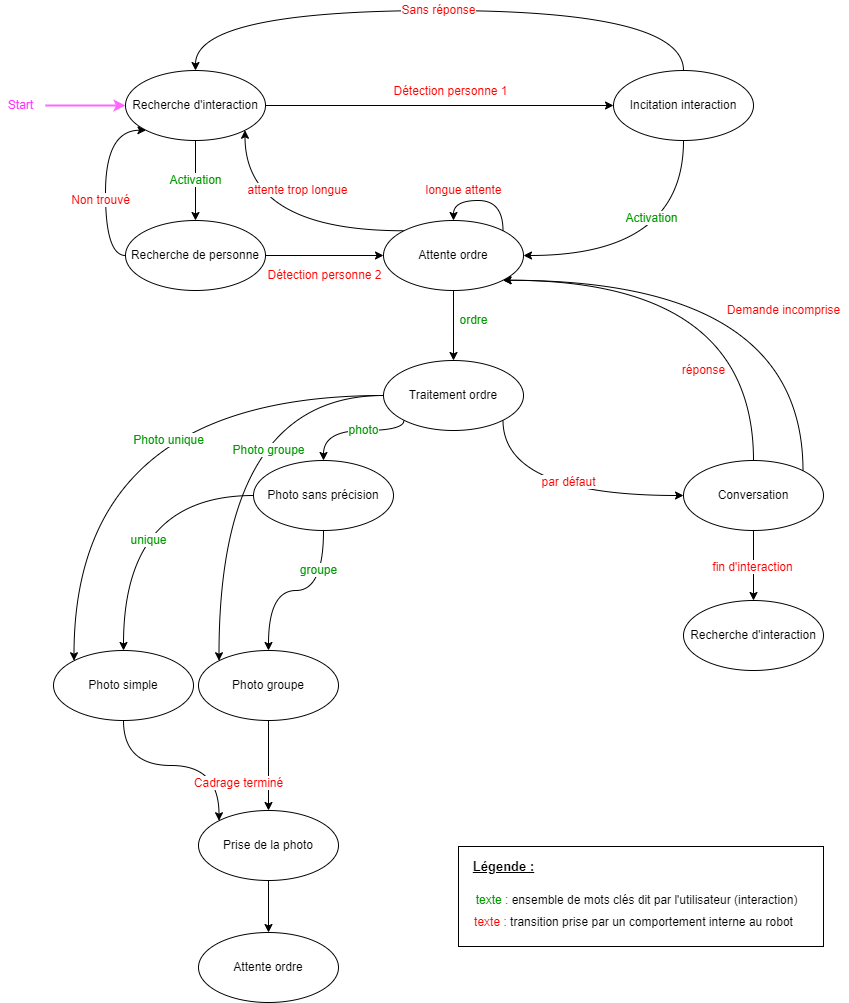
\includegraphics[scale = 0.55]{Diagramme-etats.png}
        \caption{Diagramme d'états pour les 100 ans de l'ENSEIRB}
        \label{fig:diag1}
        \end{figure}
\end{center}
\newpage


\subsection{Actions de Reachy selon les états et transitions}
Le diagramme est composé de deux parties : les états et les transitions. Sur chaque état et chaque transition, le robot réalisera des actions (mouvement, parole, ...) qui seront détaillées, d'abord pour les états, puis pour les transitions. \\

Chaque mouvement de la tête et des antennes du robot est mentionné par un \textit{nom}, le détail technique des valeurs des positions est donné en \texttt{Annexe}, section \ref{annexemouvement}, pour chacun de ses mouvements.

\subsubsection{États}
\noindent État "Recherche d'interaction" :
\begin{itemize}
    \item Synthèse vocale : Fait des petits bruits toutes les 30 secondes
    \item Mouvement: Tourne la tête pour suivre la personne la plus proche du regard sauf toutes les 3 minutes où pendant 30s le robot fera le mouvement \textit{triste}
\end{itemize} 
\ \\
État "Incitation interaction" :
\begin{itemize}
    \item Synthèse vocale : Proposer une seule fois de dire "Hey Reachy" pour commencer l'interaction
    \item Mouvement: Fait le mouvement \textit{incitation}
\end{itemize}
\ \\
État "Attente ordre" :
\begin{itemize}
    \item Mouvement: Fait le mouvement \textit{écoute}
\end{itemize}
\ \\
État "Traitement ordre" :
\begin{itemize}
    \item Mouvement: Fait le mouvement \textit{réflexion}
\end{itemize}
\ \\
État "Recherche de personne" : 
\begin{itemize}
    \item  Mouvement: Parcours de la zone possible avec recherche de visage (Cf OpenCV et direction sonore pour assister)
\end{itemize}
\ \\
Etat "Photo sans précision" :
\begin{itemize} 
    \item Synthèse vocale : Demander "Vous préférez faire une photo simple ou une photo de groupe ?"
\end{itemize}
\ \\
Etat "Photo simple" :
\begin{itemize}
    \item Mouvement: Cadrage selon OpenCV
\end{itemize}
\ \\
Etat "Photo groupe" :
\begin{itemize}
    \item Mouvement: Cadrage selon OpenCV
\end{itemize}
\ \\
Etat "Conversation" : 
\begin{itemize}
    \item Synthèse vocale/Reconnaissance vocale : Si la phrase en entrée peut être interprétée, renvoie une réponse en fonction de la phrase en entrée (couples d'entrées / sorties), sinon (si la phrase d'entrée ne correspond a rien) dit "je n'ai pas compris votre demande"
    \item Mouvement: Fait le mouvement \textit{réflexion} 
    \end{itemize}
\ \\
Etat Prise de photo :
    \begin{itemize}
    \item Synthèse vocale : Dit "je prends la photo dans 5 4 3 2 1, dites Cheeeese"
    \end{itemize}

\newpage

\subsubsection{Transitions}
\vspace{0.2cm}
\noindent Transition "Détection personne 1" :
\begin{itemize}
    \item Synthèse vocale : Après avoir trouvé, dit "Bonjour"
    \item Mouvement: Fait le mouvement \textit{content}
\end{itemize} 
\ \\
Transition "Sans réponse" :
\begin{itemize}
    \item Mouvement: Fait le mouvement \textit{triste}
\end{itemize}
\ \\
Transitions "Activation" : 
\begin{itemize}
    \item Synthèse vocale : Reachy répond "Hey, je vous écoute !" à la fin de la transition
    \item Mouvement: Fait le mouvement \textit{écoute}
\end{itemize}
\ \\
Transition "Longue attente" : 
\begin{itemize}
    \item Synthèse vocale : Dit "Je vous écoute, si vous voulez connaître l'ensemble de mes capacités demandez moi en disant "Que sais-tu faire ?""
    \item Mouvement: Fait le mouvement \textit{incitation}
\end{itemize}
\ \\
Transition "Attente trop longue" : 
\begin{itemize}
    \item Mouvement: Fait le mouvement \textit{triste}
\end{itemize}
\ \\
Transition "Non trouvé" :
\begin{itemize}
    \item Mouvement: Fait le mouvement \textit{triste}
\end{itemize}
\ \\
Transition "Détection personne 2" : 
\begin{itemize}
    \item Synthèse vocale : Dit "Oh je vous ai trouvé !"
    \item Mouvement: Fait le mouvement \textit{écoute}
\end{itemize}
\ \\
Transition "par défaut" :
\begin{itemize}
    \item Mouvement: Fait le mouvement écoute ou si l'utilisateur dit un mot triste ou gentil: 
        \begin{itemize}
        \item Mot triste → mouvement \textit{triste}
        \item Mot gentil → mouvement \textit{content}
    \end{itemize}
\end{itemize}
\ \\
Transition vers "photo unique", "photo groupe", "unique" et "groupe" :
\begin{itemize}
    \item Mouvement: Fait le mouvement \textit{écoute}
\end{itemize}
\ \\
Transition "réponse" :
\begin{itemize}
    \item None
\end{itemize}
\ \\
Transition "demande incomprise" :
\begin{itemize}
    \item Mouvement: Fait le mouvement \textit{incitation}
\end{itemize}
\ \\
Transition "Fin d'interaction" : 
\begin{itemize}
    \item Synthèse vocale Dit "Au revoir, c'était un plaisir"
    \item Mouvement: Fait le mouvement \textit{remerciement}
\end{itemize}
\ \\

\newpage

\subsection{Débuter une interaction avec le robot}
\label{begin_interact}
Avant toute interaction, le robot émettra de légers bruits (Coucou -- hmmmmm -- ehooo -- Ayee Ayee.) pour capter l'attention des individus à proximité. 
\ \\
Ensuite, deux types de début d'interaction seront développés sur le robot selon si le robot a détecté l'utilisateur avant qu'il prononce "Hey Reachy" ou non.

\begin{itemize}[leftmargin=*]
\item Dans le cas où un utilisateur prononce "Hey Reachy" avant que le robot ne le détecte. La tête se tournera vers la zone où le micro multi-directionnel identifie la voix et la reconnaissance faciale permettra d'effectuer une recherche locale d'un visage estimé "assez proche" pour être l'interlocuteur. \\
Une fois la personne détectée, Reachy lèvera les antennes vers le haut et regardera la personne pour lui faire comprendre qu'il l'a bien vue (mouvement \textit{écoute}) et qu'il est prêt à l'écouter. L'interaction pourra alors commencer. \\
Dans le cas où le robot n'identifie pas la personne qui a dit "Hey Reachy", il fera le mouvement \textit{triste}. \\

\item Dans le cas où Reachy n'entend pas "Hey Reachy", le robot cherchera des interlocuteurs et les incitera à interagir avec lui, cela constitue le deuxième cas. En effet, avant qu'une personne ne rentre en interaction avec Reachy en lui disant "Hey Reachy", le robot suivra le visage de la personne passant le plus proche et fera, tout les 3 minutes et pendant 30s, le mouvement \textit{triste}. \\

\item[] S'il détecte un utilisateur potentiel qui s'approche de lui, Reachy lèvera les antennes vers le haut et regardera la personne pour lui faire comprendre qu'il l'a bien vue et qu'il est prêt à l'écouter (mouvement \textit{incitation}). \\
Cela incitera la personne à communiquer avec le robot car il lui aura bien montré qu'il l'a détectée.\\
Après un "Hey Reachy" de la part d'un utilisateur le robot répondra "Bonjour" et l'interaction pourra commencer. \\
\end{itemize}

Dans un cas de nuisances sonores trop importantes, Reachy ne pourra pas identifier la commande vocale "Hey Reachy". Il sera alors possible pour un utilisateur extérieur de recourir à un marqueur ArUco \footnote{Les marqueurs ArUco sont identifiables avec la bibliothèque OpenCV et sont faciles à implémenter} représentant un code afin d'indiquer à Reachy certaines actions. Ces actions seront en priorité l'initiation d'interaction, équivalent à prononcer "Hey Reachy" et à la prise de photo, simple ou en groupe. \\

Afin de permettre ces différents mouvements du robot nous allons utiliser l'API \texttt{reachy-sdk} de Pollen-Robotics développée pour le robot Reachy et par conséquence programmer en utilisant le langage \textit{Python}. Elle permet de tourner la tête du robot vers la position demandée en une certaine durée. Ainsi que de bouger les antennes du robot à la vitesse souhaitée vers la position souhaitée. L'ensemble des positions, la durée et la vitesse sont paramétrables car ce sont des valeurs prises en paramètres des différentes fonctions. \\

\subsection{Gestion des ordres}
Pour donner des ordres à Reachy, les commandes devront contenir des mots clés spécifiques à chaque groupe de commandes. \\

Tout d'abord, la commande d'activation du robot nommée "Activation" dans le diagramme d'activité est paramétrable. Elle peut être définie par "Hey Reachy" , "Ok Reachy", "Bonjour Reachy", etc . Une fois l'interaction débutée comme expliqué en section \ref{begin_interact}, le robot sera en attente d'un ordre (une commande lancée par l'utilisateur). \\

De manière générale, toutes les commandes, donc ensemble de mots clés et ensemble de couples entrée/sortie, seront spécifiées dans un ou plusieurs fichier(s) \texttt{.txt} afin de pouvoir les modifier sans avoir à toucher au code. Une commande à l'intérieur d'un fichier sera de la forme : \\
\ \\
cmd : [nom de la commande] \\
. [mot clé]\\
. [mot clé]\\
...\\

Chaque commande aura donc un nom précédé de "cmd :" qui permettra à python de savoir de quelle commande il s'agit. Chaque mot clé sera précédé d'un "." et le marqueur de fin d'une liste de mots clés est "...". \\

Pour écouter les ordres, le robot fera le mouvement \textit{écoute}. Si Reachy n'a pas compris la demande de la personne, il fera le mouvement \textit{incitation} pour faire comprendre qu'il n'a pas compris et annoncera "Je n'ai pas bien compris votre demande". Aussi, si au bout d'un certain temps la personne ne pose pas de questions Reachy fera le mouvement \textit{incitation} et il proposera d'énumérer ses fonctionnalités. En cas de non interaction trop longue, le robot fera l'émotion triste avant de se remettre à chercher un autre utilisateur dans son état initial. \\

Comme indiqué sur le diagramme d'états, le robot gérera des commandes pour la prise de photos qui seront détaillées dans la partie \ref{subsec_prise_photo} et également des commandes de type conversation (cf \ref{subsec_conv_basique}). \\

A la suite d'une commande de type "Que sais-tu faire ?" , Reachy énumérera toutes ses fonctionnalités à l'utilisateur. \\

Pour réaliser la partie reconnaissance vocale, nous avons choisi d'utiliser la bibliothèque open source \\ \texttt{SpeechRecognition} ainsi que \texttt{PyAudio} qui offrent des fonctions pour l'écoute, l'enregistrement, la reconnaissance vocale et la traduction du son en texte. \\

En ce qui concerne la réalisation de la partie synthèse vocale, nous avons choisi d'utiliser la bibliothèque \texttt{pyttxs3} qui est une bibliothèque python open source qui convertit le texte en parole. Elle fonctionne hors ligne et utilise le synthétiseur vocal \texttt{eSpeak}. \\

Afin d'être utilisé durant les 100 ans de l'ENSEIRB-MATMECA le robot devra être fonctionnel dans un environnement bruyant. Il devra donc effectuer une réduction du bruit extérieur. Pour cela nous avons choisi d'utiliser la bibliothèque \texttt{wave} afin de pouvoir gérer les fichiers d'extension ".wav" ainsi que \texttt{pydub} afin de réaliser le filtrage. Chaque enregistrement sera donc stocké dans un fichier \texttt{enregistrement.wav} qui s'écrasera à chaque fois et qui sera traité avec \texttt{wave}.

\subsection{Prise de photos} \label{subsec_prise_photo}
OpenCV est une bibliothèque proposant de nombreuses fonctionnalités de vision par ordinateur, spécialisée dans le traitement d'images en temps réel. Cette bibliothèque sera utilisée pour toute utilisation des caméras du robot et permettra la reconnaissance de visages, fonctionnalité utilisée pour la prise de photo.\\ Elle permettra également d'effectuer les différents filtres photos cités dans les fonctionnalités à implémenter après les 100 ans de l'ENSEIRB-MATMECA, en section \ref{filtres}.\\

Il y a deux types distincts de prise de photos, la photo simple d'une personne et la photo d'un groupe de personnes. \\

Pour entrer dans la partie prise de photo, la commande devra contenir l'un des mots \texttt{\{"photo", "selfie"\}}. Afin de spécifier le type de la photo, il y aura deux cas de figure : si la commande contient l'un des mots \texttt{\{"moi", "me"\}}, alors ce sera une \texttt{photo simple}. Et si elle contient un ou plusieurs mots clés suivants \texttt{\{"nous", "les", "groupe", "ensemble"\}}, alors ce sera une \texttt{photo de groupe}. \\ \\
\textbf{Exemple de commandes pour une photo simple}: "Prends-moi en photo", "Hey Reachy, est ce que tu peux me prendre en selfie ?" . \\

L'utilisateur pourra demander une photo sans préciser le type de prise de photo. Dans ce cas, Reachy invitera l'utilisateur à préciser s'il souhaite une photo simple ou de groupe. L'utilisateur pourra également demander une photo simple ou une photo de groupe directement. \\ \\
Dans le cas où Reachy comprend qu'il doit faire une photo mais ne connaît pas encore quel type d'image est souhaité, il dira : "Vous préférez faire une photo simple ou une photo de groupe ?". \\

Après connaissance de la demande de prise de photos et du type de photo, Reachy ajustera la position de sa tête pour correctement cadrer la photo. Reachy cadrera la photo en conséquence du type demandé à l'aide des positions des visages obtenues grâce à la reconnaissance faciale d'OpenCV.\\

Dans le cas d'une photo simple, Reachy centrera son regard sur la position de l'unique visage à prendre en photo (le plus proche dans son champ de vision). Pour une photo de groupe, Reachy considérera tous les visages présents dans son champ de vision, il supprimera ceux estimés trop loin (trop petits par rapport à la moyenne des tailles des visages en vue) et il orientera son champ de vision vers la position moyenne des visages encore concernés.\\

Ensuite Reachy prendra la photo par enregistrement d'un instantané sur la capture vidéo avec OpenCV, et ce juste après l'annonce d'un compte à rebours : "Je prends la photo dans 5..4..3..2..1.. CHEEESE!". \\

Des images représentant un marqueur ArUco pourront être utilisées afin d'indiquer à Reachy quel type de prise de photos l'utilisateur souhaite en cas de nuisance sonore trop importante. 

\subsection{Gestion des photos}

Une fois que la photo a été prise, elle sera sauvegardée sur la mémoire du robot et ensuite affichée afin que les utilisateurs puissent la voir.

\subsubsection{Sauvegarde de la photo}

Une fois que les photos auront été prises, elles vont être enregistrées dans la mémoire du robot. Nous avons choisi de nommer la photo avec la date, l'heure et les minutes de quand elle a été prise, par exemple 08\_04\_2022-15\_45.jpg. Cependant, sa mémoire étant limitée, il nous faudra donc gérer le fait de vouloir sauvegarder une photo supplémentaire lorsque qu'il n'y aura plus assez d'espace. \\

Dans ce cas, nous favoriserons les photos récentes à celles prises précédemment. Pour cela, lorsque l'enregistrement de la photo ne pourra pas être fait par manque d'espace mémoire, un message sera envoyé pour avertir les administrateurs. Les administrateurs exécuteront une commande permettant de supprimer le nombre souhaité des plus anciennes photos (suppression à l'aide du module python \texttt{os}). Cela nous permettra de libérer assez d'espace pour enregistrer de nouvelles photos.

\subsubsection{Affichage de la photo sur un écran}

En plus de pouvoir sauvegarder les photos, un besoin spécifie que les utilisateurs puissent voir la photo une fois qu'elle aura été prise pour voir si elle leur convient. Pour cela, la photo sera affichée en temps réel sur un écran connecté au robot via un câble HDMI.

\subsection{Conversation} \label{subsec_conv_basique}

Dans un premier temps Reachy pourra entretenir une conversation très simple avec son interlocuteur. Cette conversation sera composée d'entrées et de sorties, par exemple le robot répondra "Bonjour" si on lui dit "Salut","Bonjour" ou bien "Hello". Il répondra également qu'il va très bien si on lui pose la question mais on ne pourra pas converser de manière complexe car il ne retient pas l'état de la conversation (cela sera amélioré par la suite, cf \ref{subsec_conv_avancée}). L'ensemble des couples entrées / sorties est précisé en annexe (cf \ref{subsec_couples_conv}). \\

Lorsqu'une personne sera en train de discuter avec le robot, il réagira à ce que la personne lui dit. Par exemple avoir l'air triste lorsque qu'une personne lui dira des mots considérés comme méchants et inversement content lorsqu'il entendra des mots considérés comme gentils. Si Reachy ne comprend pas les mots dit par la personne, il fera le mouvement \textit{incitation} pour faire comprendre qu'il n'a pas compris.

\subsection{Fin d'interaction}
Lorsque l'interaction sera terminée, par la demande de l'utilisateur avec une commande ou si le robot ne reçoit plus d'ordre, Reachy remerciera la personne d'avoir interagi avec lui tout en faisant le mouvement \textit{remerciement}.

\newpage

\section{Partie 2 : Après les 100 ans}
Après les 100 ans de l'\textbf{ENSEIRB-MATMECA}, nous développerons les fonctionnalités liées aux filtres sur les photos, à la recherche par Internet ainsi qu'aux conversations. Ces fonctionnalités sont détaillées ci-dessous.\\

\subsection{Diagramme d'états}
Voici le diagramme d'état de la version finale du robot :\\
\begin{center}
    \begin{figure}[!ht]
    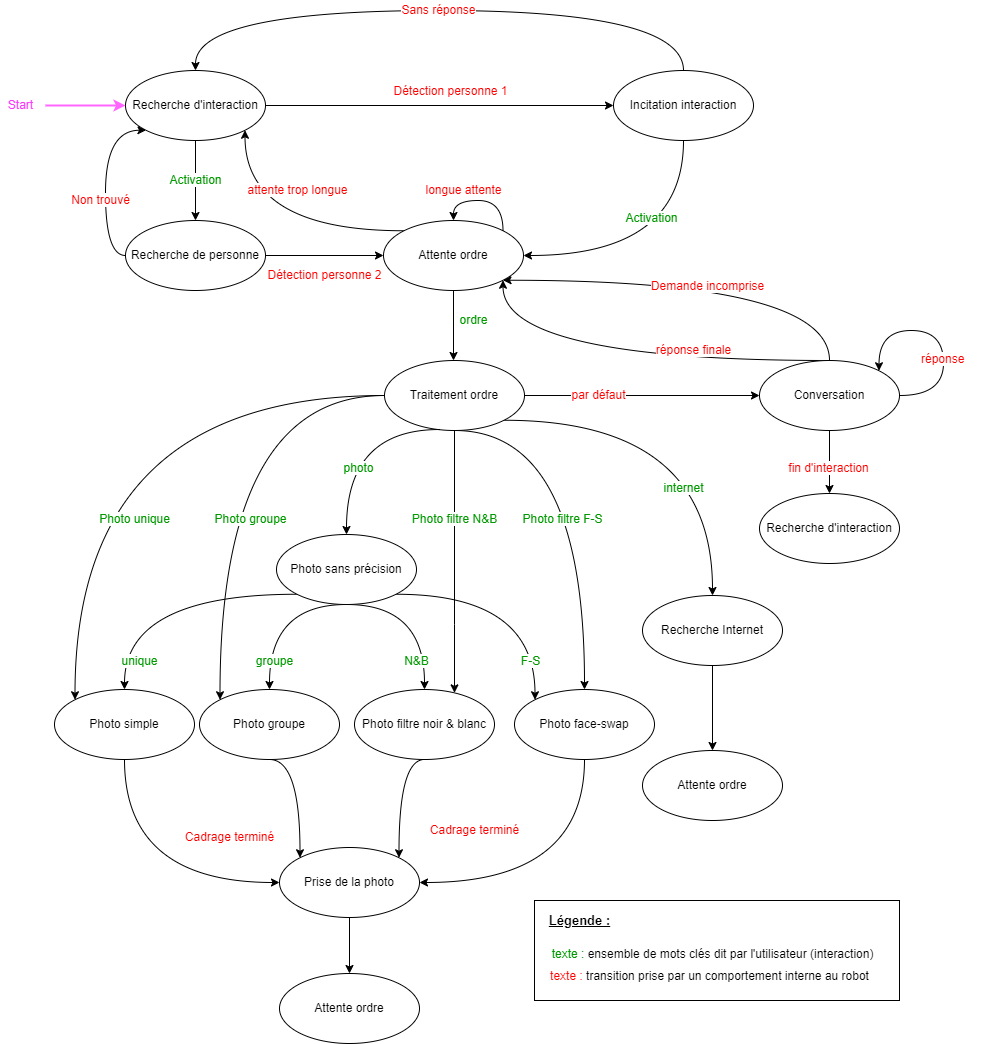
\includegraphics[width=\textwidth]{Diagramme-etat2.png}
    \caption{Diagramme d'états final du Reachy Mini}
    \label{fig:diag1}
    \end{figure}
\end{center}
\newpage

\newpage

\subsection{Filtres sur les photos}\label{filtres}
\noindent Additionnellement à la prise de photos, des filtres pourront être appliqués à ces photos :
\begin{itemize}
    \item Le premier filtre consistera à faire de l'échange de visages, où les deux visages les plus proches sur la photo seront échangés.
    \item Le second filtre consistera à mettre la photo en noir et blanc.
\end{itemize}

Si le développement est assez avancé, les filtres pourront être appliqués en direct sur la capture vidéo, et une dernière fonctionnalité consistera à indiquer la similarité des deux visages les plus proches sur la photo. \\
Ces fonctionnalités seront implémentées à l'aide de l'API d'OpenCV.

\subsection{Recherche Internet}
L'un des besoins fonctionnels du client est la recherche sur internet, notamment pour des conditions de surf à une date et un lieu précis. Ainsi nous utiliserons les API \texttt{webbrowser} et \texttt{request} afin de réaliser des recherches selon des urls et extraire des données trouvées sur une page web. \\

Si l'utilisateur réalise une demande contenant un des mots clés \texttt{\{condition, surf\}}, alors le robot lui demandera pour quel jour \texttt{J} et quel lieu \texttt{L} réaliser la recherche des conditions de surf.
Reachy pourra ainsi effectuer une recherche internet en complétant l'url correctement avec \texttt{J} et \texttt{L}, et en extraire les informations importantes qu'il dira à l'utilisateur par l'intermédiaire de la synthèse vocale. \\

Ces recherches seront effectuées sur le site \texttt{https://www.surf-report.com/}, et le robot ex+plicitera la hauteur des vagues, la température sur place ainsi que le temps. \\

Lorsque la personne aura demandé d'effectuer une recherche, il fera le mouvement \textit{réflexion} ainsi que le mouvement \textit{incitation} s'il n'a pas compris la demande de la personne.

\subsection{Conversations plus interactives} \label{subsec_conv_avancée}
Après les 100 ans de l'ENSEIRB la partie conversation du robot devra être améliorée. Le robot devra être capable de tenir une conversation simple avec son interlocuteur, il devra notamment pouvoir tenir une conversation du type : \\
\ \\
- (I) Bonjour.\\
- (R) Hello !\\
- (I) Qui es-tu ? \\ 
- (R) Je suis Reachy et vous ? \\ 
- (I] Je m'appelle Test. \\
- (R) Enchanté Test\\
- (I) Comment vas-tu ? \\
- (R) Je me porte bien merci, et vous Test ? \\
- (I) Je vais très bien \\
- (R) Super \\
- (I) Que fais-tu ici ? \\ 
- (R) Je propose mes services de photographe pour l'évènement d'aujourd'hui. \\
\ \\

Pour cela nous allons continuer avec des mots clés mais en ajoutant une notion de mémoire de l'état de la conversation et comme l'indique le nouveau diagramme d'états on ne sort pas forcément directement de l'état Conversation à chaque commande. La figure \ref{fig_conv_avance} résume les interactions ajoutées : 

    \begin{figure}[!ht]
        \begin{center}
        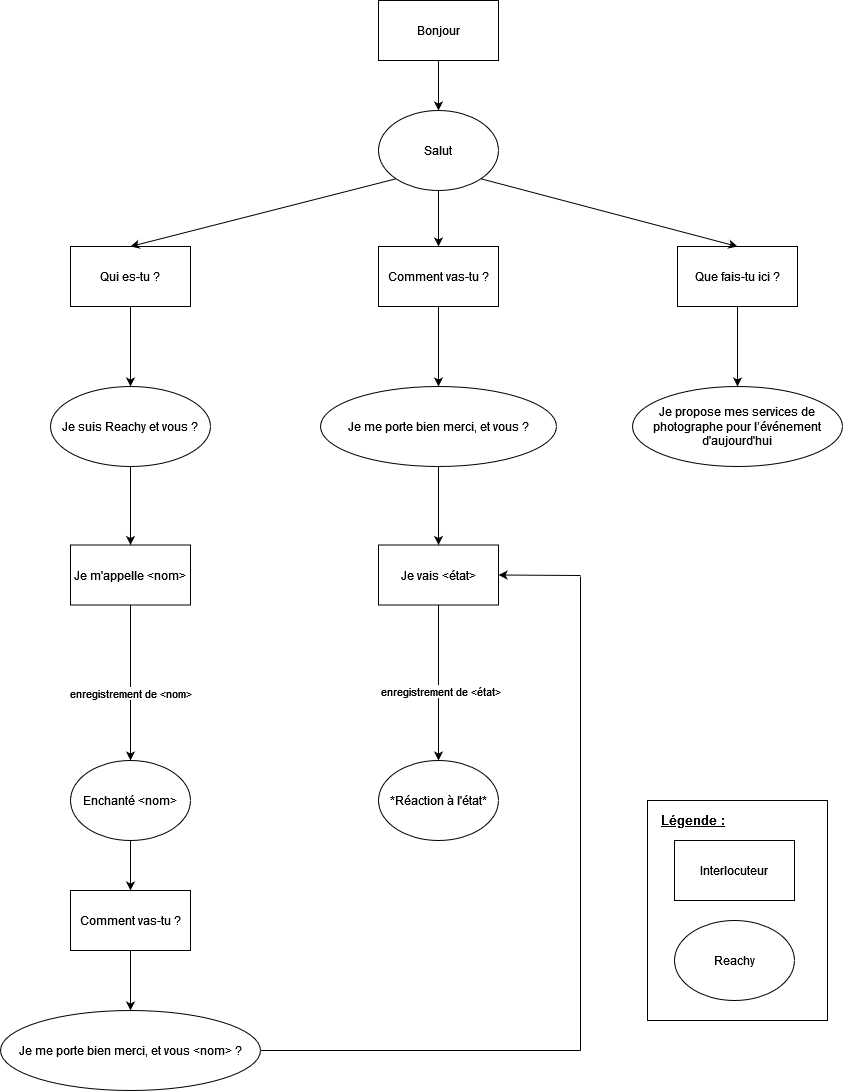
\includegraphics[scale = 0.5]{Schema-Conversation.png}
        \caption{Schéma des Conversations avancées}
        \label{fig_conv_avance}
        \end{center}
    \end{figure}
\newpage

On peut voir les rectangles de la Figure \ref{fig_conv_avance} comme des noms d'ensembles de mots clés qui sont spécifiés en annexe (cf \ref{annexemotsclés}). Les ellipses quant à elles peuvent être vues comme les sorties car ce seront les phrases dites par le robot. \\
\ \\
Cette partie conversation avancée pourra être densifiée de manière optionnelle, voici ce qui pourra être rajouté :
\begin{itemize}
    \item Des couples entrée/sortie marrants comme par exemple : "Je suis ton père" / "Vous devez confondre, je ne suis pas Luke Skywalker". 
    \item Des devinettes avec un fichier contenant un ensemble de couples question/réponses, lues grâce aux commandes natives de python. L'interlocuteur pourra demander une devinette, le robot choisira un couple question/réponses, posera la question et vérifiera la conformité de la réponses avec celle qu'il connaît (mots clés pour les réponses).
    \item Des questions de culture générale sur le même modèle que les devinettes.
    \item Des blind tests sur des extraits audio de 10 secondes sur le même modèle que les devinettes.
\end{itemize}

\section{Deux cas d'utilisation}
Les principales fonctionnalités du robot peuvent être mises en application à l'aide de cas d'utilisation. La couverture du diagramme d'état est un indice de la force de ces cas d'utilisation. Il serait possible d'obtenir une pleine couverture en réalisant des cas d'utilisation pour chaque type de photo, et chaque type de conversation (recherche internet ou non, conversation simple ou non). Nous développerons ici les deux principaux cas qui permettent une couverture suffisamment élevée.
\subsection{Interaction directe}
\begin{figure}[!ht]
    \centering
    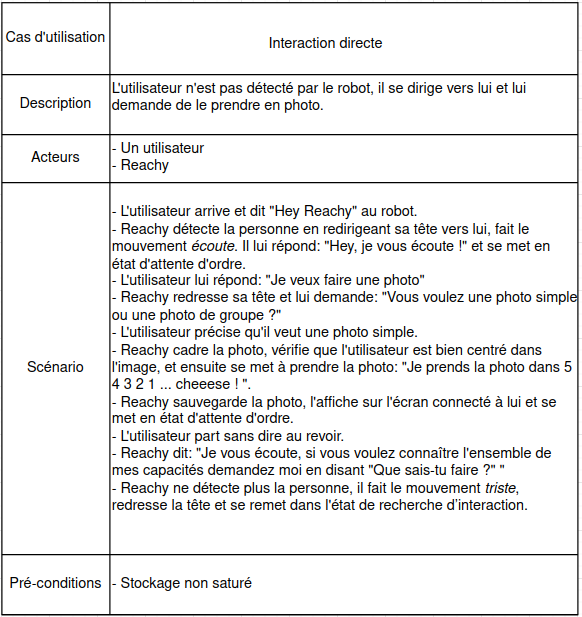
\includegraphics[scale = 0.52]{use_case1.png}
    \caption{$1^{er}$ cas d'utilisation}
\end{figure}
Dans un premier cas, on considère un utilisateur qui n'est pas détecté par le robot. Il adresse la parole à Reachy en lui disant "Hey Reachy". Reachy recherche donc l'utilisateur en tournant la tête vers lui. \\

Une fois la personne détectée, le robot, fait le mouvement \textit{écoute}, et répond "Hey, je vous écoute !" . Il se met alors en attente d'un ordre de l'utilisateur. Ce dernier demande "Je veux faire une photo". Reachy redresse sa tête et demande : "Vous préférez faire une photo simple ou une photo de groupe ?". L'utilisateur précise qu'il veut faire une photo simple. \\

Le robot se met donc à cadrer la photo afin d'avoir l'utilisateur au milieu de l'image. Ensuite, il rentre en phase de prise de photo et lance le compte à rebours pour capturer la photo en disant : "Je prends la photo dans 5..4..3..2..1..CHEEESE !". Une fois la photo prise, elle sera sauvegardée est affichée sur l'appareil connecté au robot.\\ 

Reachy se retrouve alors de nouveau en attente d'un ordre. L'utilisateur est parti sans dire au revoir, donc le robot considère l'attente trop longue, et précise "Je vous écoute, si vous voulez connaître l’ensemble de mes capacités demandez moi en disant ”Que sais-tu faire ?"". Comme l'utilisateur n'est plus là, le robot fait le mouvement \textit{triste} puis redresse la tête pour pour la recherche de visages qui est le premier état.

\subsection{Interaction par détection de visage}
\begin{figure}[!ht]
    \begin{center}
        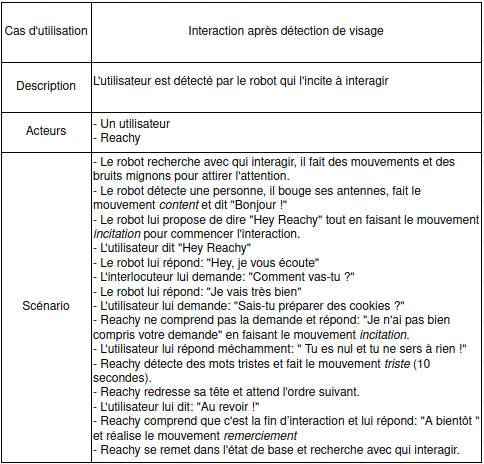
\includegraphics[scale = 0.62]{use_case2.png}
        \caption{$2^{`eme}$ cas d'utilisation}
    \end{center}
\end{figure}
Dans ce deuxième cas, l'interaction est débutée par la détection d'un utilisateur par Reachy. \\

Le robot recherche une personne tout en faisant des mouvements et des bruits mignons pour attirer l'attention. Il détecte donc une personne à proximité, et se met à agiter les antennes avec le mouvement \textit{content} et dit "Bonjour". \\

Il propose ensuite au client de dire "Hey Reachy" tout en faisant le mouvement \textit{incitation} pour commencer l'interaction. L'utilisateur déclenche effectivement l'interaction en disant "Hey Reachy" et Reachy répond "Hey, je vous écoute". Ensuite l'interlocuteur demande "Comment vas-tu ?", le robot lui répond alors "Je vais très bien". \\

Ensuite l'utilisateur demande : "Sais-tu préparer des cookies ?". Reachy dans ce cas ne comprend pas et répond gentiment "Je n'ai pas bien compris votre demande" en faisant le mouvement \textit{incitation}. \\

L'utilisateur enchaîne ensuite la conversation en disant "Tu es nul de toute façon !". Le robot identifie donc que ce sont des mots tristes, et fait le mouvement \textit{triste} pendant 10 secondes. \\

Après il redresse sa tête et attend le prochain ordre ou la prochaine réplique. Le client lui dit "A bientôt", Reachy comprend donc que le client s'écarte. Il lui répond "A bientôt", réalise le mouvement \textit{remerciement} et se remet dans l'état de base qui est la recherche de personne.

\newpage

\section{Tâches et livrables}
Dans cette partie, nous détaillerons les étapes de la réalisation technique, ensuite, nous présenterons les diagrammes de Gantt et nous listerons tous les livrables.
\subsection{Les étapes de réalisation techniques}
\subsubsection{La reconnaissance faciale}
\begin{itemize}
    \item \textbf{Identification de visage} [ 2 jours ] : Obtention en capture vidéo d'une structure de donnée renseignant des informations sur la position des visages et affichage à l'écran clarifiant la réussite de l'identification (carré autour des têtes, points particuliers du visage, ...)
    \item \textbf{Suivi de visage} [ 1-2 semaine(s) ] : Obtention des angles horizontaux et verticaux entre la normale à la caméra et le centre des visages de la capture vidéo. Adaptation des angles ressortis pour un suivi optimal du visage le plus proche.
    \item \textbf{Cadrage pour prise de photo} [ 1-2 semaine(s) ] : Prise en compte des visages les plus proches, puis recherche du barycentre des centres des visages pour diriger le regard vers ce barycentre en guise de cadrage
    \item \textbf{Échange de visages} [ 1-3 semaines moyennant qualitativité ] :
    \begin{itemize}
        \item \indent [ 3 jours ] : Échange des deux têtes les plus proches (par les carrés les entourant)
        \item \indent [ 5 jours ] : Échange des deux visages les plus proches (par une méthode plus poussée). Les visages n'auront pas les bonnes proportions
        \item \indent [ 1 semaine ] : Correction des proportions et adaptation des traits faciaux
        \item \indent [ 5 jours ] : Adaptation de la colorimétrie des visages échangés
    \end{itemize}
    \item \textbf{Mise en noir et blanc} [ 1 jour ] : Colorimétrie de la photo transformée en noir et blanc
    \item \textbf{Similarité de visages} [ 5 jours ] : Pourcentage de similarité des deux visages les plus proches sur la photo
\end{itemize}

\subsubsection{Mouvement du robot}
\begin{itemize}
    \item \textbf{Premier mouvement de tête et des antennes séparément} [ 1-3 jour(s) ] : effectuer un mouvement quelconque avec la tête, de même pour les antennes.
    \item \textbf{Faire avoir des émotions} [ 1-2 semaine(s) ] : Combiner des mouvements de la tête et des antennes pour faire comme si le robot avait des émotions ("content", "triste", "pensif", ...).
    \item \textbf{Faire avoir des émotions à partir d'une position initiale connue} [ 1-2 semaines ] : Lui faire avoir les émotions dans l'orientation où la tête était avant; pour cela lui donner les déplacements sous la forme de 3 angles qui seront ensuite transformés sous la forme de coordonnées cartésiennes.
    \item \textbf{Mouvement lié aux photos} [ 1 semaine ] : Récupérer, de la partie photo, les valeurs des angles dont le robot doit bouger pour pouvoir prendre puis cadrer la photo.
    \item \textbf{Mouvement permettant de suivre les personnes} [ 1 semaine ] : Tourner la tête pour qu'elle soit toujours en face de la personne qui, soit interagit avec Reachy, soit la personne la plus proche lorsque le robot n'interagit avec personne.
    \item \textbf{Mouvement pour se tourner vers le son} [ 1 semaine ] : Récupérer, de la partie reconnaissance vocale d'où vient le son, les valeurs des angles dont le robot doit bouger pour pouvoir plus facilement trouver où se trouve la personne qui parle.
    \item \textbf{Fluidifier les mouvements} [ 2 semaines ] : Faire que les mouvements soient plus fluides et plus naturels afin qu'ils se rapprochent plus de ceux d'un être humain.
\end{itemize}

\subsubsection{Gestion des ordres}
\begin{itemize}
    \item \textbf{Transcription de la voix en texte} [ 1 jour ] : écouter l'interlocuteur et transformer ses paroles en texte.
    \item \textbf{Atténuation du bruit extérieur moyen} [ 8-13 jour(s) ] : atténuer les bruits extérieurs afin de se concentrer sur la source principale du son et pouvoir être utilisé dans un environnement moyennement bruyant
    \item \textbf{Mise en place d'un système de conversation basique} [ 3-5 jour(s) ] : le robot doit pouvoir répondre à de commandes telles que "Bonjour" ou bien "Qui es-tu ?".
    \item \textbf{Gestion des marqueurs ArUco} [ 5-8 jours ] : reconnaître un marqueur ArUco, le retranscrire en entier et l'associer à une commande existante pour pouvoir être utilisé sans reconnaissance vocale.
    \item \textbf{Atténuation du bruit extérieur fort} [ 9-14 jour(s) ] : atténuer les bruits extérieurs afin de se concentrer sur la source principale du son et pouvoir être utilisé dans un environnement fortement bruyant.
    \item \textbf{Amélioration du système de conversation} [ 12-15 jour(s) ] : le robot doit pouvoir tenir une conversation basique (cf \ref{subsec_conv_avancée}).
\end{itemize}

\subsubsection{Synthèse vocale}
\begin{itemize}
    \item \textbf{Conversion d'un texte en son} [ 1 jour ] : faire saisir un texte et le transformer en parole.
    \item \textbf{Faire parler le robot} [ 4 jours ] : vérifier les sorties audio du robot et ses paramètres et le faire parler.
    \item \textbf{Faire des petits bruits} [ 4 jours ] : faire produire des petits bruits mignons et des phrases pour attirer l'attention. 
    \item \textbf{Amélioration de la voix} [ 1 semaine ] : améliorer la voix du robot.
\end{itemize}

\subsubsection{Recherche Internet}
\begin{itemize}
    \item \textbf{Reconnaissance des informations nécessaires} [ 5 jour ] : Transformer les paramètres énoncés par l'utilisateur en url de recherche.
    \item \textbf{Extraction des informations nécessaires} [ 1 semaine ] : Extraire sur la page web les informations utiles (hauteur de vagues, température, temps).
    \item \textbf{Énoncer les informations} [ 1 semaine ] : Énoncer ces informations à l'utilisateur de façon précise et concise.
\end{itemize}

\subsection{Diagrammes de Gantt}
Toutes ces étapes de la réalisation peuvent être résumées dans un diagramme, nommé diagramme de Gantt, qui permet de définir des dates précises concernant l'évolution du robot. De plus, cela permet la visualisation de livrables qui seront rendus pour réaliser des cycles de construction du projet et retour du client. Nous avons découpé ce diagramme en deux sous diagrammes, un concernant avant les 100 ans de l'\textbf{ENSEIRB-MATMECA} et un après.
\begin{center}
    \begin{figure}[!ht]
        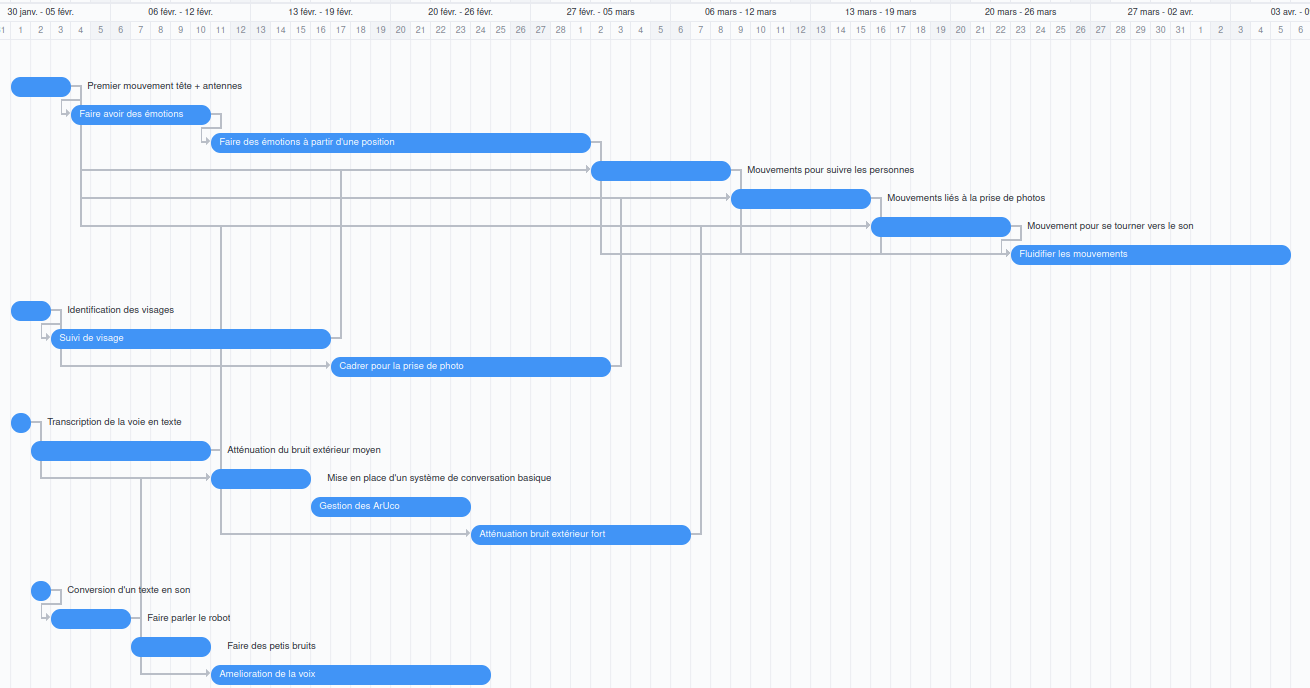
\includegraphics[width=\textwidth]{GANTT_avant_100_ans.png}
        \caption{Diagramme de Gantt avant les 100 ans}
        \label{fig:gantt_avant}
        \end{figure}
\end{center}

\begin{center}
    \begin{figure}[!ht]
        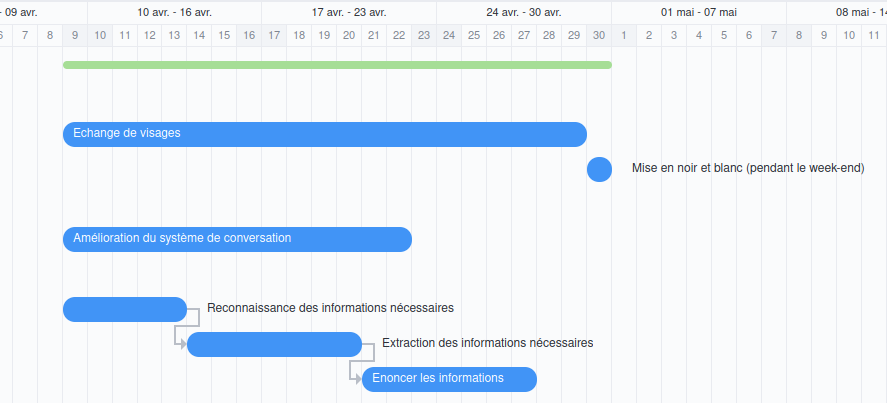
\includegraphics[width=\textwidth]{GANTT_apres_100_ans.png}
        \caption{Diagramme de Gantt après les 100 ans}
        \label{fig:gantt_apres}
        \end{figure}
\end{center}

\newpage

\subsection{Livrables}
Voici les livrables qui se dégagent du diagramme de Gantt :

\subsubsection{"Hello World" [07/02/22]}
L'objectif de ce livrable est de fournir un robot capable d'effectuer les actions les plus basiques de chacun des axes majeurs de son fonctionnement. Il devra donc pouvoir effectuer un mouvement simple, reconnaître un visage, entendre une voix et la transformer en texte et dire une phrase quelconque. 

\subsubsection{Full Interaction [16/02/22]}
L'objectif de ce livrable est de fournir un robot capable de lier ses axes majeurs de fonctionnement entre eux de manière basique. Il devra donc reconnaître une personne, bouger en conséquence, écouter une voix et répéter la phrase dite.

\subsubsection{Le robot communique avec émotions [25/02/22]}
L'objectif de ce livrable est de fournir un robot capable d'avoir une conversation basique avec l'utilisateur tout en montrant ses émotions.

\subsubsection{Le robot sait prendre des photos [11/03/22]}
L'objectif de ce livrable est de fournir un robot capable de cadrer une ou plusieurs personnes pour les prendre en photo.

\subsubsection{Le robot communique et prend des photos [18/03/22] }
L'objectif de ce livrable est de fournir un robot capable d'avoir une conversation plus dynamique avec l'utilisateur après l'avoir détecté et capable de le cadrer et le prendre en photo.

\subsubsection{100 ans de l'ENSEIRB [01/04/22]}
L'objectif de ce livrable est de fournir un robot capable d'effectuer tout ce qui est spécifié dans la partie \ref{sec_100_ans}.
Les mouvements du robot sont plus fluides et le robot propose différents filtres et fonctionnalités lors de la prise d'une photo.

\subsubsection{Système de conversation amélioré [23/04/22]}
Le robot peut entretenir une conversation avec un utilisateur de manière fluide et interactive (mémorisation du prénom, action en fonction du sentiment)

\subsubsection{Recherche internet pour des conditions de surf [30/04/22]}
Le robot permet d'annoncer les conditions de surf pour une date et un lieu précis selon la demande de l'utilisateur.

\subsubsection{Full version [07/05/22]}
L'objectif de ce livrable est de fournir un robot capable d'effectuer tout ce qui est spécifié dans ce cahier des charges. Les filtres sur les photos auront donc été rajoutés.

\newpage

\section{Webographie}

\begin{itemize}
    \item{[1]} \url{https://www.pollen-robotics.com}
    \item{[2]} \url{https://github.com/pollen-robotics/reachy-sdk}
    \item{[3]} \url{https://docs.pollen-robotics.com}
    \item{[4]} \url{https://docs.python.org/fr/3/library/wave.html}
    \item{[5]} \url{https://opencv.org}
    \item{[6]} \url{https://pypi.org/project/SpeechRecognition}
    \item{[7]} \url{https://pypi.org/project/PyAudio}
    \item{[8]} \url{https://pypi.org/project/pydub}
    \item{[9]} \url{https://pypi.org/project/pyttsx3}
    \item{[10]} \url{https://towardsdatascience.com}
    \item{[11]} \url{https://docs.python.org/3/library/webbrowser.html}
    \item{[12]} \url{https://fr.python-requests.org/en/latest}
    
\end{itemize}
\newpage
\section{Annexe} \label{annexe}

\subsection{Définition des positions} \label{annexemouvement}
Une position est la combinaison d'un mouvement de la tête et des antennes.
Le mouvement de la tête est réalisé en fonction de 3 coordonnées \texttt{(x, y, z)} qui déterminent un point de l'espace où Reachy regarde. Pour se rendre dans une certaine position, il est possible de déterminer la durée que prendra le mouvement. Le mouvement des antennes est caractérisé par une vitesse limite des antennes ainsi que deux angles qui correspondent au positionnement de chaque antenne. \\

Nous détaillons ici les différentes positions de notre robot, dont nous pourrons factoriser le code.
\begin{center}
    \begin{tabular}{| c | c | c | c | c | c |}
        \hline
        Position & Cordonnées & Durée & Angle Antenne Gauche & Angle Antenne Droite & Vitesse Antennes \\
        \hline
        écoute & (0.5, 0, -0.05) & 2.0 & 0 & 0 & / \\
        triste & (0.5, 0, -0.3) & 2.0 & 140.0 & -140.0 & 70 \\
        content & (0.5, 0, -0.05) & 2.0 & $\pm$20.0 & $\pm$20.0 & 300 \\
        incitation & (0.5, 0, 0.05) & 1.0 & 35.0 & -35.0 & 70 \\
        réflexion & (0.5, 0.15, 0.15) & 1.0 & -40.0 & 40.0 & 70 \\
        remerciement & (0.5, 0, -0.20) & 0.5 & -40.0 & 40.0 & 70 \\
        \hline
    \end{tabular}
\end{center}

Le mouvement content est un mouvement où les antennes alternent leur position. Ainsi, elles alterneront en différé entre -20 et +20.
Le mouvement remerciement correspond à la mise en position écoute, puis remerciement, puis écoute. Ainsi, le robot baisse la tête comme pour saluer son interlocuteur.

\subsection{Ensembles de mots clé} \label{annexemotsclés}
Nous avons choisi de définir des ensembles de mots pour les commandes. La transition dans le diagramme d'états est faite selon le type de transition que l'on a choisi. \\ \\
Voici les différentes transitions :
\begin{itemize}
    \item {\color{red}"one in"} = si la phrase de l'utilisateur contient un mot de l'ensemble de mots.
    \item {\color{red}"all in"} = si la phrase de l'utilisateur contient tous les mots de l'ensemble de mots.
    \item {\color{red}"n in"} = si la phrase de l'utilisateur contient n mots de l'ensemble de mots.
\end{itemize}
\ \\
Ensemble "Hey Reachy" {\color{red}("all in")}:
\begin{itemize}
    \item Hey 
    \item Reachy
\end{itemize}
\ \\
Ensemble "Photo" {\color{red}("one in")}:
\begin{itemize}
    \item photo
    \item selfie
    \item photographie
    \item photographier
    \item cliché
\end{itemize} 
\ \\
Ensemble "unique" {\color{red}("one in")}:
\begin{itemize}
    \item moi
    \item me 
\end{itemize}
\ \\
Ensemble "Groupe" {\color{red}("one in")}:
\begin{itemize}
    \item nous
    \item groupe
    \item ensemble
    \item les \\
\end{itemize}


Dans le diagramme il y a une transition directe entre "traitement ordre" et "photo simple" ou "photo groupe". En fait il s'agit d'une double analyse de la phrase de l'utilisateur par Reachy.
\\
Si la phrase est "prend moi en photo" on passera d'abord dans l'état "Photo sans précision" avec la détection de "photo" puis on passera dans l'état "Photo simple" avec la détection de "moi". \\
\ \\
Exemples "Photo unique":
\begin{itemize}
    \item Prend {\color{red}moi} en {\color{red}photo}.
    \item Tu peux {\color{red}me} prendre en {\color{red}photo} ? 
    \item Tu peux {\color{red}me photographier} ?
    \item Prend {\color{red}moi} en {\color{red}selfie}.
\end{itemize}
\ \\
Exemples "Photo groupe"
\begin{itemize}
    \item Prend {\color{red}nous} en {\color{red}photo}
    \item Prend une {\color{red}photographie} de {\color{red}groupe}
    \item Fait un {\color{red}cliché} de notre {\color{red}groupe}
    \item Tu peux nous {\color{red}prendre} en photo {\color{red}ensemble} ?
\end{itemize}
\ \\
Passons maintenant aux ensembles de mots clés concernant les fonctionnalités implémentées après les 100 ans de l'ENSEIRB. \\

Ensemble "N\&B" {\color{red}("one in")}:
\begin{itemize}
    \item noir et blanc
    \item monochrome \\
\end{itemize}

Ensemble "F-S" {\color{red}("one in")}:
\begin{itemize}
    \item échangeant
    \item échange \\
\end{itemize}

Exemples "Photo N\&B"
\begin{itemize}
    \item Prend une {\color{red}photo monochrome}
    \item Prend une {\color{red}photo} en {\color{red} noir et blanc} \\
\end{itemize}

Exemples "Photo F-S"
\begin{itemize}
    \item Prend une {\color{red}photo} avec un {\color{red}échange} de visage
    \item Prend une {\color{red}photo} en {\color{red}échangeant} nos visages\\
\end{itemize}

Ensemble "internet" {\color{red}("one in")}:
\begin{itemize}
    \item conditions
    \item surf \\
\end{itemize}

Ce cas est différent car il demande une date et un lieu on devra donc repérer une date qui pourra être spécifiée de cette façon, on repère plusieurs cas : \\

Cas pas de date: \\
On recherche les conditions de surf le jour actuel.\\
\underline{Exemple :} "quelles sont les conditions de surf à Lacanau ?" \\

Cas une date peu précise (jour de la semaine)  : \\
On recherche les conditions de surf correspondantes au jour de la semaine précisé le plus proche de la date actuelle.
\underline{Exemple :} "quelles sont les conditions de surf Samedi à Lacanau ?" \\

Cas une date précise : \\
On recherche les conditions de surf le jour spécifié. \\
\underline{Exemple :} "quelles sont les conditions de surf le Jeudi 27 Janvier à Lacanau ?" \\

Cas pas de lieu : \\
On recherche les conditions de surf au Grand Crohot. \\
\underline{Exemple :} "quelles sont les conditions de surf aujourd'hui ?" \\

Cas un lieu précis: \\
On recherche les conditions de surf lieu précisé. \\
\underline{Exemple :} "quelles sont les conditions de surf aujourd'hui à Lacanau ?" \\

\subsection{Couple pour la conversation basique} \label{subsec_couples_conv}
Nous n'avons pas pour objectif de permettre une longue conversation avec le Reachy,  il s'agirait plutôt de couple d'entrées et de sorties sans garder en mémoire l'état de la conversation actuelle. Le Reachy utilisera la bibliothèque \texttt{random} afin de pouvoir gérer l'aléatoire, ici une sortie est présentée sous la forme du texte de sortie suivi du pourcentage de chance de renvoyer cette sortie entre parenthèse.\\
\ \\
Entrée :
\begin{itemize}
    \item Bonjour 
    \item Coucou
    \item Salut
    \item Hello
\end{itemize}
Sortie : \\
\begin{itemize}
    \item Bonjour (50\%)
    \item Salut (50\%)
\end{itemize}
\ \\
Entrée :
\begin{itemize}
    \item Comment vas-tu ?
    \item Comment ça va ?
\end{itemize}
Sortie :
\begin{itemize}
    \item Très bien et vous ? (100\%)
\end{itemize}
\ \\
Entrée (mots clés ; {\color{red}"one in"}): 
\begin{itemize}
    \item gentil
    \item sympathique
    \item mignon
    \item beau
\end{itemize}
Sortie :
\begin{itemize}
    \item Merci (100\%) + Mouvement : content
\end{itemize}
\ \\
Entrée (mots clés ; {\color{red}"one in"}): 
\begin{itemize}
    \item méchant
    \item moche
    \item inutile
    \item nul
\end{itemize}
Sortie :
\begin{itemize}
    \item Mouvement : \textit{triste}
\end{itemize}
\ \\
Entrée incomprise \\
Sortie :
\begin{itemize}
    \item Je n'ai pas bien compris votre demande ? (100\%)
\end{itemize}

\subsection{Ensembles de phrases/mots clés pour la conversation avancée}

Ensemble "Qui es-tu ?" {\color{red}("one in")}:
\begin{itemize}
    \item Qui es-tu ?
    \item Qu'es-tu ?\\
\end{itemize}

Ensemble "Je m'appelle [nom]?" {\color{red}("one in")}:
\begin{itemize}
    \item Je m'appelle [nom]
    \item Je suis [nom]
    \item{[nom] \\} 
\end{itemize}

L'ensemble "Je m'appelle [nom]" fait suite à "Qui es-tu ?" donc Reachy sait que son interlocuteur va lui transmettre son nom c'est pourquoi si la réponse est composée d'un seul mot, Reachy l'interprétera comme le nom de son interlocuteur. \\

Ensemble "Que fais-tu ici ?" : \\
Cet ensemble est un peu particulier, il est composé de 2 ensembles de mots clés à détecter. En effet, la phrase doit contenir l'un des mots suivants : 
\begin{itemize}
    \item Fais
    \item Pourquoi
\end{itemize}
Ainsi que l'un de ces mots :
\begin{itemize}
    \item ici
    \item là \\
\end{itemize}

Ensemble "Comment vas-tu ?" {\color{red}("one in")}:
\begin{itemize}
    \item Comment vas-tu ?
    \item Ça va ? 
    \item Tout va bien ? \\
\end{itemize}

Ensemble "Je vais [état]" {\color{red}("one in")}:
\begin{itemize}
    \item Je vais [état]
    \item{[état] \\}
\end{itemize}

L'ensemble "Je vais [état]" se rapproche de "Je m'appelle [nom]" puisque Reachy s'attend ici aussi au type de réponse puisqu'il fait suite à une question de Reachy, un état seul peut donc suffire. \\

La suite fait la liste des états possibles détectés par Reachy ainsi que les mots clés associés. \\

Ensemble "bien" {\color{red}("one in")}:
\begin{itemize}
    \item bien
    \item très bien
    \item super
    \item ça va
    \item en forme \\
\end{itemize}

Réponse de Reachy (Réaction à l'état) : "Super" + mouvement \textit{content}\\

Ensemble "mal" {\color{red}("one in")}:
\begin{itemize}
    \item pas (afin de détecter les états du type "ça ne va pas")
    \item mal
    \item triste 
    \item fatigué \\
\end{itemize}

Réponse de Reachy (Réaction à l'état) : mouvement \textit{triste}
